Finden Sie die Funktion $y(x)$, deren Graph durch die Punkte $(0,0)$
und $(1,0)$ geht, die das Integral
\begin{align*}
A(y)
&=
\int_{0}^{1} y(x)^2\,dx
\intertext{maximiert und für die ausserdem die Bedingung}
B(y)
&=
\int_{0}^{1}
y'(x)^2
\,dx
=
C
\end{align*}
erfüllt.


\begin{loesung}
Die Lagrange-Funktionen der beiden Funktionale sind
\begin{align*}
F(x,y,y') &= y^2          &&\text{für $A(y)$}\\
G(x,y,y') &= y^{\prime 2} &&\text{für $B(y)$.}
\end{align*}
Von beiden muss jetzt der Gradient gebildet werden, also die linke
Seite der Euler-Lagrange-Differentialgleichung.
Für $F$ ist dies
\[
\frac{\partial F}{\partial y}(x,y(x),y'(x))
-
\frac{d}{dx}\frac{\partial F}{\partial y'}(x,y(x),y'(x))
=
2y(x),
\]
für $G$ ist es
\[
\frac{\partial G}{\partial y}(x,y(x),y'(x))
-
\frac{d}{dx}\frac{\partial G}{\partial y'}(x,y(x),y'(x))
=
-\frac{d}{dx}(2y'(x))
=
-2y''(x).
\]
Nach der Methode der Lagrange-Multiplikatoren muss jetzt die Funktion
${\color{darkred}y(x)}$ und eine Zahl ${\color{darkred}\lambda}\in\mathbb{R}$
so gefunden werden, dass
\begin{align}
2{\color{darkred}y(x)}&=-2{\color{darkred}\lambda y}''{\color{darkred}(x)}
\label{buch:aufgabe:501:eqn:dgl}
\\
\int_{x_1}^{x_2} {\color{darkred}y}\mathstrut'{\color{darkred}(x)}^2\,dx &= C
\label{buch:aufgabe:501:eqn:integral}
\\
{\color{darkred}y}(0) &= 0
\label{buch:aufgabe:501:eqn:rb1}
\\
{\color{darkred}y}(1) &= 0
\label{buch:aufgabe:501:eqn:rb2}
\end{align}
Als Erstes lösen wir die Differentialgleichung~\eqref{buch:aufgabe:501:eqn:dgl}
in der Form
\[
y''(x) = -\frac{1}{\lambda} y(x).
\]
Je nach Vorzeichen von $\lambda$ gibt es verschieden mögliche Lösungen.

Wir versuchen zunächst den Ansatz $y(x)=e^{\omega x}$ und bekommen
\[
\omega^2e^{\omega x} = -\frac{1}{\lambda} e^{\omega x},
\]
und damit $\omega=\pm1/\!\sqrt{-\lambda}$.
Diese Lösung existiert nur dann, wenn $\lambda<0$ ist.
Die Funktion $y(x)$ ist daher eine Linearkombination 
\[
y(x) = a_+ e^{x/\!\sqrt{-\lambda}} + a_- e^{-x/\!\sqrt{-\lambda}}.
\]
Diese Funktion muss jetzt ausserdem die Randbedingungen erfüllen.
Wir setzen daher $0$ und $1$ ein und erhalten das homogene lineare
Gleichungssystem
\begin{equation}
\renewcommand{\arraycolsep}{3pt}
\begin{array}{lclcl}
a_+                        &+& a_-                         &=& 0 \\
a_+e^{1/\!\sqrt{-\lambda}} &+& a_-e^{-1/\!\sqrt{-\lambda}} &=& 0
\end{array}
\label{buch:aufgabe:501:eqn:homogen}
\end{equation}
Für die Koeffizienten $a_+$ und $a_-$.
Die Koeffizientenmatrix hat die Determinante
\[
e^{1/\!\sqrt{-\lambda}}-e^{-1/\!\sqrt{-\lambda}}
=
e^{1/\!\sqrt{-\lambda}}(1-e^{-2/\!\sqrt{-\lambda}}).
\]
Da die Exponentialfunktion $e^\xi$ nur für $\xi=0$ den Wert
1 annimmt, verschwindet die Klammer niemals und damit auch die
Determinante nicht.
Das Gleichungssystem \eqref{buch:aufgabe:501:eqn:homogen}
kann daher nur die triviale Lösung $a_+=a_-=0$ haben.
Dann ist aber die Funktion $y(x)=0$, d.~h.~die Nebenbedingung
\eqref{buch:aufgabe:501:eqn:integral} kann nicht erfüllt werden, 
der Ansatz mit Exponentialfunktionen führt nicht auf eine Lösung.
Folglich muss $\lambda>0$ sein.

Im Fall $\lambda>0$ sind die Funktionen
\[
\sin(x/\!\sqrt{\lambda})
\qquad\text{und}\qquad
\cos(x/\!\sqrt{\lambda})
\]
Lösungen der Differentialgleichung.
Die allgemeine Lösung ist daher eine Linearkombination
\[
y(x)
=
a \cos(x/\!\sqrt{\lambda})
+
b \sin(x/\!\sqrt{\lambda}).
\]
Jetzt setzen wir die Randbedingung an der Stelle $x=0$ ein und erhalten
\[
0
=
y(0)
=
a.
\]
An der Stelle $x=1$ folgt dann
\[
0=y(1)
=
b\sin(1/\!\sqrt{\lambda}).
\]
Da die Nullstellen der Sinusfunktion die ganzzahligen Vielfachen von $\pi$
sind, folgt
\[
1/\!\sqrt{\lambda} = k\pi
\qquad\Rightarrow\qquad
\lambda = \frac{1}{k^2\pi^2}
\]
für $k\in\mathbb{N}$.
Damit ist jetzt gefunden, dass
\[
y(x) = b \sin k\pi x
\]
ist.
Jetzt muss $b$ nur noch so bestimmt werden, dass die
Nebenbedingung~\eqref{buch:aufgabe:501:eqn:integral} erfüllt ist.
Dies ist die Gleichung
\begin{align*}
C
&=
\int_0^1 y'(x)^2\,dx
\\
&=
\int_0^1 b^2 k^2\pi^2 \cos^2 k\pi x\,dx
\\
&=
b^2k^2\pi^2 \int_0^1 \cos^2 k\pi x\,dx
=
\frac{b^2k^2\pi^2}2
\qquad
\Rightarrow
\qquad
b
=
\frac{\!\sqrt{2C}}{k\pi}.
\end{align*}
%
% cos2.tex -- Integral von cos^2
%
% (c) 2021 Prof Dr Andreas Müller, OST Ostschweizer Fachhochschule
%
\documentclass[tikz]{standalone}
\usepackage{amsmath}
\usepackage{times}
\usepackage{txfonts}
\usepackage{pgfplots}
\usepackage{csvsimple}
\usetikzlibrary{arrows,intersections,math}
\begin{document}
\def\skala{1}
\begin{tikzpicture}[>=latex,thick,scale=\skala]

\fill[color=blue!10] (0,0) rectangle (5,5);
\fill[color=blue!20] plot[domain=0:1,samples=100]
	({5*\x},{5*cos(540*\x)*cos(540*\x)})
	-- (5,0) -- (0,0) -- cycle;
\draw[color=blue] plot[domain=0:1,samples=100]
	({5*\x},{5*cos(540*\x)*cos(540*\x)});
\draw[->] (0,-0.05) -- (0,5.5) coordinate[label={right:$y$}];
\draw[->] (-0.05,0) -- (5.5,0) coordinate[label={$x$}];
\draw (5,-0.05) -- (5,0.05);
\node at (5,-0.05) [below] {$1$};
\node at (0,-0.05) [below] {$0$};
\node at (-0.05,5) [left] {$1$};
\node at (-0.05,0) [left] {$0$};
\node[color=blue] at (2.5,5) [above] {$y(x)=\cos^2 k\pi x$};

\end{tikzpicture}
\end{document}

%
Die Berechnung des Integrals von $\cos^2 k\pi x$ ist einfach, wenn man
berücksichtigt, dass der Graph des Integranden aus Symmetriegründen
das Einheitsquadrat halbiert (siehe
Abbildung~\ref{buch:nebenbedingungen:aufgabe:501:fig:cos2}).
Die Lösungen sind jetzt also die Funktionen
\[
y_k(x)
= 
\frac{\!\sqrt{2C}}{k\pi}
\sin k\pi x.
\]
%
% yk.tex
%
% (c) 2024 Prof Dr Andreas Müller
%
\begin{figure}
\centering
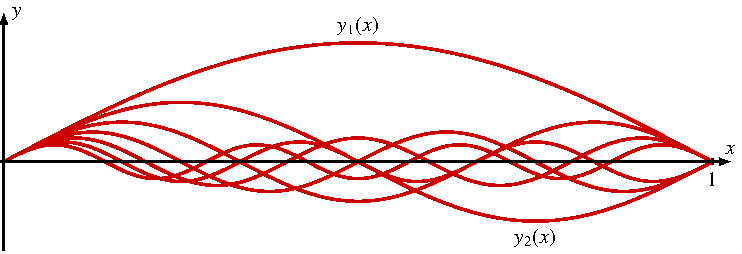
\includegraphics{chapters/050-nebenbedingungen/images/yk.pdf}
\caption{Lösungen des Variationsproblems von Aufgabe~\ref{501}.
\label{buch:nebenbedingungen:aufgabe:501:fig:yk}}
\end{figure}

Die Lösungen sind in Abbildung~\ref{buch:nebenbedingungen:aufgabe:501:fig:yk}
dargestellt.

Der Wert des Integrals $A(y)$ kann jetzt ebenfalls bestimmt werden, es
ist
\begin{align*}
A(y_k)
&=
\int_0^1 y_k(x)^2\,dx
=
\int_0^1 b^2\sin^2 k\pi x\,dx
=
\frac{2C}{k^2\pi^2} \int_0^1 \sin^2k\pi x\,dx
=
\frac{C}{k^2\pi^2}.
\end{align*}
Da $k\in\mathbb{N}$ sein muss, wird das Maximum bei $k=1$ erreicht und
hat den Wert $C/\pi^2$.
\end{loesung}
